\documentclass[border=8pt]{standalone}
\usepackage{tikz}
\usetikzlibrary{arrows.meta,positioning,calc}
\begin{document}
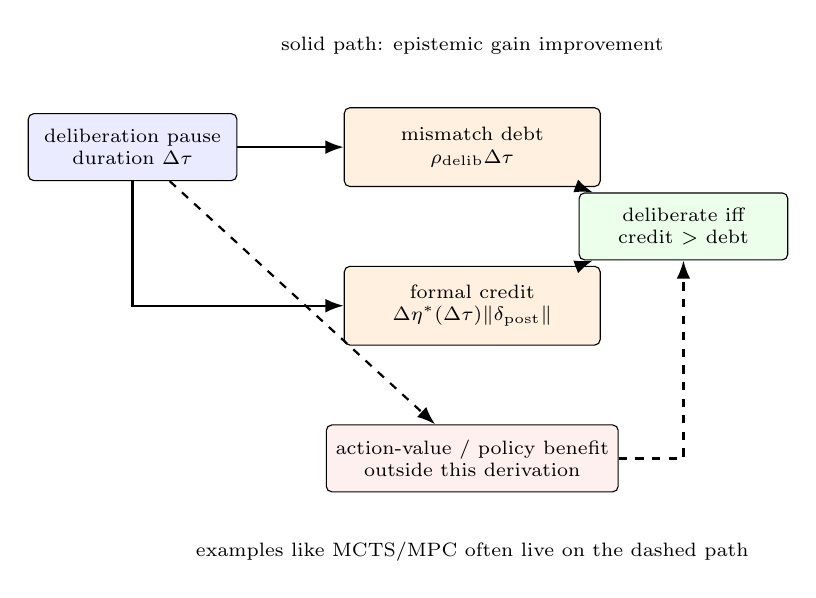
\begin{tikzpicture}[
  box/.style={draw, rounded corners=2pt, align=center, minimum width=2.65cm, minimum height=0.85cm, font=\scriptsize},
  ledger/.style={draw, rounded corners=2pt, align=center, minimum width=3.25cm, minimum height=1.0cm, font=\scriptsize, fill=orange!12},
  note/.style={align=center, font=\scriptsize},
  arr/.style={-Latex, thick},
  dasharr/.style={-Latex, thick, dashed}
]

\node[box, fill=blue!8] (pause) {deliberation pause\\duration $\Delta\tau$};
\node[ledger, right=1.35cm of pause] (cost) {mismatch debt\\$\rho_{\rm delib}\Delta\tau$};
\node[ledger, below=1.0cm of cost] (benefit) {formal credit\\$\Delta\eta^\ast(\Delta\tau)\|\delta_{\rm post}\|$};
\node[box, fill=green!8, right=1.35cm of $(cost)!0.5!(benefit)$] (rule)
  {deliberate iff\\credit $>$ debt};

\draw[arr] (pause) -- (cost);
\draw[arr] (pause) |- (benefit);
\draw[arr] (cost) -- (rule);
\draw[arr] (benefit) -- (rule);

\node[box, fill=red!6, below=1.0cm of benefit, minimum width=3.25cm] (outside)
  {action-value / policy benefit\\outside this derivation};
\draw[dasharr] (pause) -- (outside);
\draw[dasharr] (outside) -| (rule);

\node[note, above=0.55cm of cost] {solid path: epistemic gain improvement};
\node[note, below=0.5cm of outside] {examples like MCTS/MPC often live on the dashed path};

\end{tikzpicture}
\end{document}
